\paragraph{Administrator Bedienoberfläche}
\ac{aem} bietet einige Werkzeuge an, mit deren Hilfe das System administriert und erweitert werden kann. Zum Beispiel wäre hier eine Bedienoberfläche für die OSGi-Verwaltung und für administrative Eingriffe in das \ac{crx} zu nennen.\\
Entwickler müssen häufig Eigenschaften und Knoten des \ac{crx} editieren. Eine Möglichkeit, dies zu bewerkstelligen, wäre mit dem Tool CRXDE Lite, welches ebenfalls über den Webbrowser erreichbar ist, und es wird bei \ac{aem} per Standard mit installiert. \\
\autoref{img:crxde} zeigt einen Beispielknoten innerhalb einer lauffähigen \ac{aem}-Webanwendung, welche für Lernzwecke mit dem \ac{aem} installiert werden kann.

\begin{figure}[H]
	\begin{center}
		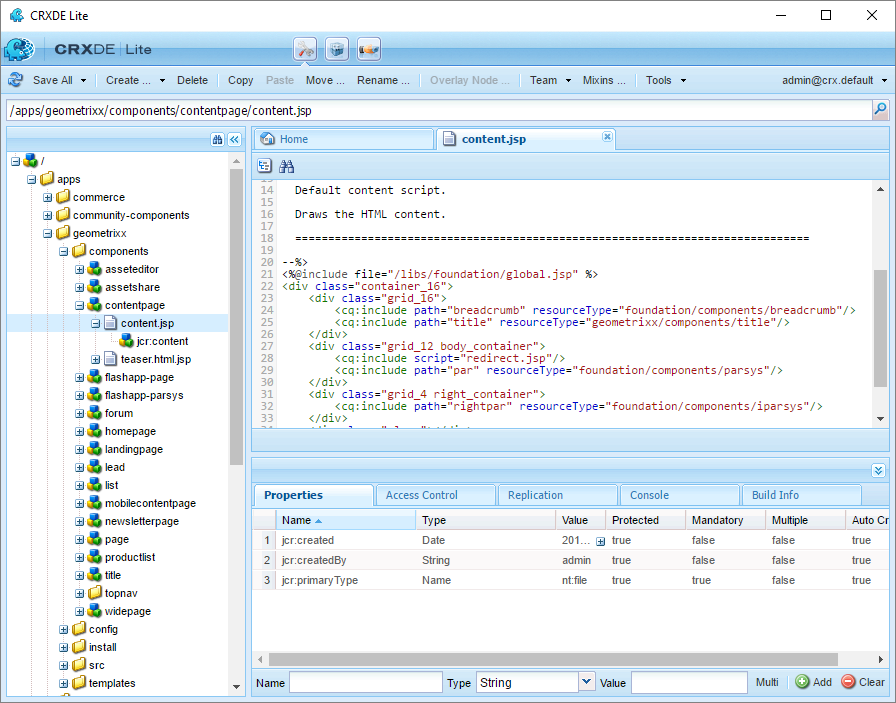
\includegraphics[width=1\textwidth]{crxde.png}
		\caption{CRXDE Lite}
		\label{img:crxde}
	\end{center}
\end{figure}

Wie sich der Abbildung entnehmen lässt, wird die Baumstruktur auf der linken Seite angezeigt. Unten rechts sind die Eigenschaften des gewählten Knotens zu sehen und oben rechts lassen sich Templates und Java-Dateien bearbeiten.